\section{Descripción del problema}\label{intro}
% Historia de los CADS y la imagen médica
Antes de profundizar en la descripción del problema que abordaremos en este proyecto final de carrera (PFC), hablaremos acerca del contexto en el que se inscribe.\medskip\par

La introducción de la imagen médica digitalizada ha transformado la práctica clínica. 
En la década de los 60 \cite{journals/cmig/Doi07} comienzan los esfuerzos por desarrollar líneas de investigación para el diagnóstico asistido por ordenador (CAD), pero no es hasta la década de los 80 cuando la tecnología permite que esta disciplina despegue. Solo como apunte para mostrar el impacto que tiene  el desarrollo de la imagen médica: la detección de cáncer de mama ha incrementado aproximadamente en un 10\% \cite{journals/cmig/Nishikawa07}, aunque podemos encontrar muchos otros ejemplos \cite{johnston1994effects, doi:10.1117/12.877968, kundel1975interpreting, Fujita:2008:CDE:1456710.1456735}.\medskip\par

% Historia de los PACs y DICOM
El formato de estas imágenes es crucial para el desarrollo de la investigación. Los Sistemas de Adquisición y Procesado de Imagen médica (PACs) \cite{huang2010pacs} contienen tanto el software como el hardware necesario para el tratamiento de la imagen médica.  Los principales elementos que forman los PACs son \cite{pianykh2012digital}:
\begin{itemize}
	\item \textit{Dispositivos de adquisición}: permiten la captura de la imagen médica. Estos dispositivos no tiene que compartir la misma tecnología de captura. Por lo que encontramos dispositivos de adquisición de imágenes como:
	\begin{itemize}
		\item Ultrasonidos.
		\item Resonancia magnética.
		\item Tomografía Axial Computarizada (TAC).
		\item Rayos X.
		\item \ldots
	\end{itemize}
	\item \textit{Archivos de la imagen médica}: servidores donde almacenar las imágenes.
	\item \textit{Estaciones de trabajo}: estaciones dónde los profesionales leen y trabajan con estas imágenes. 
\end{itemize}

 En la figura \ref{fig:pacs} vemos un esquema de los sistemas de adquisición y procesamiento de la imagen médica que acabamos de describir.\par
\begin{figure}[ht]
\centering
\includegraphics[scale=0.6]{./imgs/esquemas/pacs.pdf}
\caption{Componentes principales de los PACs}
\label{fig:pacs}
\end{figure}

\medskip\par

Y aunque en los inicios de estos sistemas cada fabricante comenzó desarrollando su propio formato para el majejo de las imagenes \cite{huang2011short, lemke2011short}, no tardaron en aflorar problemas derivados de la falta de un estándar para compartir y estudiar estas. Por este motivo surge en 1983 el estándar  Digital Imaging and Communication in Medicine (DICOM).\medskip\par

DICOM es un estándar \cite{bidgood1992introduction} desarrollado por el colegio Estadounidense de Radiología (ACR) y la asociación Nacional de Fabricantes eléctricos (NEMA), especifica no  solo el formato de las imágenes sino también como deben ser almacenadas, los protocolos para el intercambio de las mismas. \par
En los veinte años de vida el estándar no ha dejado de crecer. Se han desarrollado más de 160 suplementos al mismo que completan las carencias detectadas en su uso y se adaptan a las nuevas tecnologías. Entre el 2006 y el 2013, los temas en los que se ha centrado el foco de atención son la mejora en las tecnologías para la adquisición de las imágenes y los informes estructurados asociados a estas.\cite{dicomtrends}.
Precisamente de estos dos temas dan pie a dos líneas de investigación bien diferenciados en la literatura \cite{torres2012improving}:
\begin{itemize}
	\item \textit{Imagen médica}: cómo almacenar y procesar la información de las imágenes médicas. 
	\item \textit{Informes médicos}: informes estructurados con información de las imágenes.  
\end{itemize}
\medskip\par

Es precisamente en esta segunda rama de la investigación en la que nos centraremos en este PFC. Concretamente dentro del estándar DICOM, se especifica una extensión para tratar con los informes médicos estructurados, se trata del estándar DICOM-SR \cite{clunie2000dicom}, del cual relegamos una definición más en profundidad en el aparatado \ref{dicomSR}.\par
La correcta estructuración de los informes permite organizar el conocimiento sobre las imágenes, permitiendo comparar imágenes de manera precisa mediante métodos cuantificables, y con esta información mejorar el diagnóstico.  Estos informes estructurados, (así como la imagen médica) ofrece a los profesionales sanitarios herramientas de apoyo a la medicina basada en evidencias \cite{Sackett19973, Darlenski2010553, Elphick2004525}, y con los datos necesarios para entrenar a los sistemas de diagnostico asistidos por ordenador.\medskip\par

En la literatura podemos encontrar diferentes esfuerzos por mejorar el tratamiento del conocimiento contenido en los informes médicos\cite{BlanquerEspert:2009:COV:1528937.1529213,journals/jbi/TorresQEH12, journals/jamia/Tirado-RamosHL02}  y de la utilidad del uso de los informes DICOM-SR. \par
Pero lo que es evidente es que para que los estudios derivados de los informes médicos estructurados (DICOM-SR) sean eficaces necesitamos disponer de un conjunto amplio y preciso de estos. Aunque el uso de métodos estadísticos nos ayuda a paliar en  este problema, los modelos que se generen a partir de los datos y por extensión las conclusiones a las que pudiéramos llegar, serían en el mejor de los casos imprecisos. \par
Paradójicamente, nos encontramos con un cuello de botella en la adquisición de los datos en los informes DICOM-SR a partir de la imagen médica, ya que este proceso debe hacerlo un profesional. Rellenar formularios electrónicos pude ser una tarea tediosa, por lo que en la actualidad se emplea el reconocimiento del habla  para transcribir los informes de los profesionales como texto plano. Pero el lenguaje natural es impreciso por lo que se necesitan herramientas para aplicar la estructura de un informe DICOM a este texto plano \cite{sevenster2012aut, 9227155, citeulike:191295}. \medskip\par

Y es en este punto dónde encontramos el problema que queremos abordar. Necesitamos informes médicos estructurados, pero su adquisición es demasiado costosa y poco productiva de la manera tradicional, ya que la interacción requerida para que el usuario introduzca los datos es poco intuitiva y monótona, y las herramientas para aplicar la estructura del informe médico DICOM-SR al texto plano se ciñen a tipos de imagen concretos (Radiografías, radiologías,\ldots) debido a la complejidad de interpretar correctamente el lenguaje natural.\medskip\par

El otro elemento que nos hace falta para terminar de definir el problema, nos vincula con la solución que propondremos en el apartado \ref{solucion}, y es que afortunadamente las nuevas tecnologías nos ofrecen nuevas posibilidades. La interacción con los terminales móviles inteligentes han demostrado ser mucho más intuitiva y amigable para todo tipo de usuarios.\par
En los últimos años podemos encontrar trabajos que han comenzado a introducir terminales móviles inteligentes en el campo médico con resultados satisfactorios. \cite{journals/jdi/ChoudhriR11,20359897,journals/jdi/TangLLC04}\bigskip\par

Recapitulando, la existencia de estándares en la imagen médica ha facilitado el desarrollo de distintas líneas de investigación que han revolucionado la práctica clínica. \par
Los informes estructurados son una valiosa fuente de información médica, pero su adquisición requiere aumentar la carga de trabajo de los profesionales. \par
Los terminales móviles ofrecen nuevas formas de interactuar con los usuarios de manera más intuitiva, y su uso en el ámbito médico se ha probado productivo. \par


\section{Solución propuesta}\label{solucion}
La solución que se propone para el problema que hemos descrito en el apartado anterior, explota las ventajas que nos ofrecen los terminales móviles. Lo que se propone es desarrollar una aplicación que permita generar automáticamente una aplicación para terminales móviles inteligentes con el sistema operativo Android a partir de plantillas de los informes médicos estructurados (DICOM-SR).\medskip\par

Partimos de ficheros que sigan el estándar para informes médico DICOM-SR con la definición de la plantilla del tipo de informe en el que estamos interesados. Estos ficheros contienen información  acerca del tipo de informe, así como de todos los campos que deben estar presentes en el mismo; también contiene para cada campo información acerca del tipo, de las propiedades de cardinalidad, verificación de los mismos y posibles valores a asignar.\par

A partir de estos ficheros, extraeremos la información de los mismos y generamos el código necesario para crear un aplicación para terminales móviles inteligentes Android. Una vez hemos generado todos los ficheros necesarios (interfaz, modelo de clases, interacciones entre la interfaz de usuario, \ldots), los integraremos en el esqueleto de una aplicación Android estándar para este propósito, y de este modo tendremos el informe estructurado, convertido en una aplicación para terminales inteligentes.\par
En la figura \ref{fig:basic_schema}, podemos ver un esquema muy básico de la solución propuesta: la entrada del sistema es el fichero con la plantilla DICOM-SR, que se pasa a la aplicación en python que hemos desarrollado y esta genera una aplicación en Android con los datos del informe estructurado DICOM-SR. Entraremos en más detalles acerca de la arquitectura y la justificación de los detalles técnicos de la solución en los siguientes apartados.\bigskip\par

\begin{figure}[ht]
\centering
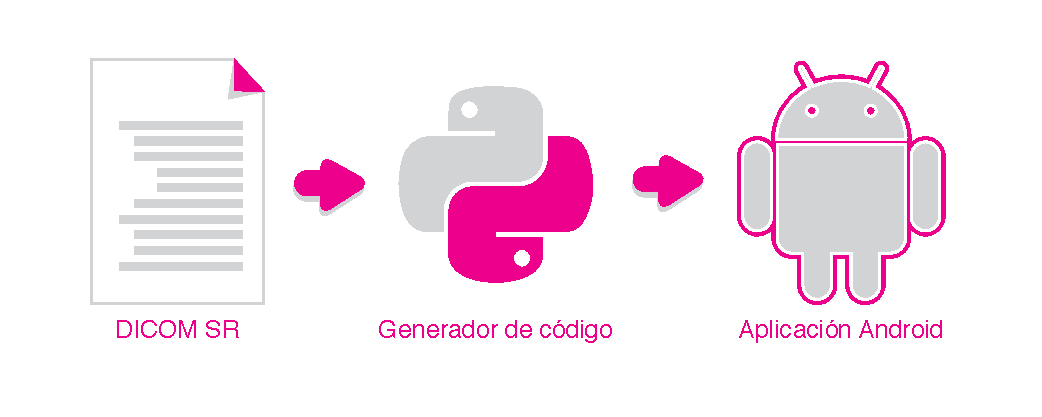
\includegraphics[scale=0.6]{./imgs/esquemas/simple.pdf}
\caption{Esquema básico}
\label{fig:basic_schema}
\end{figure}

El objetivo que pretendemos lograr con esta solución es claro: hacer uso de una interfaz de usuario muy intuitiva característica de los terminales móviles inteligentes, para interactuar con el usuario. Cuanto más podamos simplificar el trabajo del usuario a la hora de codificar los informes, más probablemente el profesional introduzca un número mayor de informes y de una forma más productiva. \medskip\par
La solución propuesta tiene varios puntos fuertes, que son los siguientes:
\begin{itemize}
\item Se trata de una solución \textit{genérica}. Independientemente del tipo de informe médico podemos de manera automática crear una aplicación Android que lo soporte.
\item Es \textit{adaptable} a los cambios en la plantilla DICOM-SR. Si añadimos nuevos campos, o modificamos el tipo de los mismos, la aplicación que se generaría cambiaría adaptándose a los cambios realizados en el informe.
\item Es \textit{configurarle}, ya el usuario podría decidir la configuración más intuitiva para él/ella.
\item La \textit{ubicuidad} de los terminales Android aporta al usuario la posibilidad al personal médico de comenzar la introcción de los datos en una pantalla táctil y continuar en una tableta. 
% TODO: Añadir la cita a los léxicos
\end{itemize}
\medskip\par

En definitiva, se trata de una solución que busca que los profesionales médicos introduzcan los datos de las imágenes que analicen en los informes médicos estructurados de tipo DICOM-SR  de una manera rápida e intuitiva. Los datos específicos de cada paciente introducidos por el profesional interactuando con la aplicación Android, se guardarán de nuevo en el formato estándar DICOM-SR. 